\documentclass[10pt,a4paper,oneside]{99_fhnwreport}

%%%%%%%%%%%%%%%%%%%%%%%%%%%%%%%%%%%%%%%%%%%%%%%%%%%%%%%%%%%%%%%%%%%%%%%%%%%%%%%%
% basic font and language packages
%%%%%%%%%%%%%%%%%%%%%%%%%%%%%%%%%%%%%%%%%%%%%%%%%%%%%%%%%%%%%%%%%%%%%%%%%%%%%%%%
%\usepackage[left=20mm,right=20mm,top=20mm,bottom=20mm]{geometry}
\usepackage[T1]{fontenc} % font encoding
\usepackage{lmodern} % font latin modern
\usepackage[utf8]{inputenc} % input encoding
\usepackage[ngerman]{babel} % english and german word spelling
\usepackage[babel, german=swiss]{csquotes} % german cites
%\usepackage[babel, english=british]{csquotes} % english cites

%%%%%%%%%%%%%%%%%%%%%%%%%%%%%%%%%%%%%%%%%%%%%%%%%%%%%%%%%%%%%%%%%%%%%%%%%%%%%%%%
% style packages
%%%%%%%%%%%%%%%%%%%%%%%%%%%%%%%%%%%%%%%%%%%%%%%%%%%%%%%%%%%%%%%%%%%%%%%%%%%%%%%%
\usepackage{hyperref} % use hyperlinks in table of contents
\hypersetup{colorlinks=true,urlcolor=blue,linkcolor=black} % define hyperlink colors
\usepackage{verbatim} % don't interpret latex symbols (source code)
\usepackage{enumerate} % numbered items
\usepackage{graphicx} % use figures
\usepackage{subfigure} % more than one figure in the same place
\usepackage{booktabs} % create tables
\usepackage{multirow} % create tables
\usepackage{cite} % citations
\usepackage{pdflscape} % allow landscape sites in pdf documents
\usepackage{pdfpages} % include pdf files

%%%%%%%%%%%%%%%%%%%%%%%%%%%%%%%%%%%%%%%%%%%%%%%%%%%%%%%%%%%%%%%%%%%%%%%%%%%%%%%%
% mathematical packages
%%%%%%%%%%%%%%%%%%%%%%%%%%%%%%%%%%%%%%%%%%%%%%%%%%%%%%%%%%%%%%%%%%%%%%%%%%%%%%%%
\usepackage{amsmath} % formula
\usepackage{amsfonts} % formula
\usepackage{amssymb} % formula
\usepackage{amsthm} % formula
\usepackage{listings} % source code formatting

%%%%%%%%%%%%%%%%%%%%%%%%%%%%%%%%%%%%%%%%%%%%%%%%%%%%%%%%%%%%%%%%%%%%%%%%%%%%%%%%
% optional parameters
%%%%%%%%%%%%%%%%%%%%%%%%%%%%%%%%%%%%%%%%%%%%%%%%%%%%%%%%%%%%%%%%%%%%%%%%%%%%%%%%
\bibliographystyle{IEEEtran}
\graphicspath{{./graphics/}{./appendix/}}

% source code parameters
\lstset{numbers=left, numberstyle=\tiny, numbersep=6pt}
\lstset{captionpos=b, tabsize=4, basicstyle=\small, xleftmargin=0mm, xrightmargin=0mm}

%%%%%%%%%%%%%%%%%%%%%%%%%%%%%%%%%%%%%%%%%%%%%%%%%%%%%%%%%%%%%%%%%%%%%%%%%%%%%%%%
% debugging parameters
%%%%%%%%%%%%%%%%%%%%%%%%%%%%%%%%%%%%%%%%%%%%%%%%%%%%%%%%%%%%%%%%%%%%%%%%%%%%%%%%
%\usepackage{todonotes}
%\overfullrule=1em

%%%%%%%%%%%%%%%%%%%%%%%%%%%%%%%%%%%%%%%%%%%%%%%%%%%%%%%%%%%%%%%%%%%%%%%%%%%%%%%%
% document settings
%%%%%%%%%%%%%%%%%%%%%%%%%%%%%%%%%%%%%%%%%%%%%%%%%%%%%%%%%%%%%%%%%%%%%%%%%%%%%%%%
%\title{Title\\\large Undertitle}
\title{
	\textsc{\LARGE{Technisches Pflichtenheft}}\\[10mm]
	\textsc{\LARGE{Dojo - Mehr als nur ein Museumsguide}}
}

\author{}

\date{\today}

%%%%%%%%%%%%%%%%%%%%%%%%%%%%%%%%%%%%%%%%%%%%%%%%%%%%%%%%%%%%%%%%%%%%%%%%%%%%%%%
% pictures
%\begin{figure}[htb]
%\includegraphics[width=\textwith]{image1.png}
%\figcaption{image1} % picture caption
%\label{fig:image1}
%\end{figure}
%
%(Abb. \ref{fig:image1})
%%%%%%%%%%%%%%%%%%%%%%%%%%%%%%%%%%%%%%%%%%%%%%%%%%%%%%%%%%%%%%%%%%%%%%%%%%%%%%%

%%%%%%%%%%%%%%%%%%%%%%%%%%%%%%%%%%%%%%%%%%%%%%%%%%%%%%%%%%%%%%%%%%%%%%%%%%%%%%%
% equation
%\begin{equation}
%X_{1,2} = \frac{-b \pm \sqrt{b^{2}-4ac}}{2a}
%\label{eq:equation1}
%\end{equation}
%%%%%%%%%%%%%%%%%%%%%%%%%%%%%%%%%%%%%%%%%%%%%%%%%%%%%%%%%%%%%%%%%%%%%%%%%%%%%%%

%%%%%%%%%%%%%%%%%%%%%%%%%%%%%%%%%%%%%%%%%%%%%%%%%%%%%%%%%%%%%%%%%%%%%%%%%%%%%%%
% table
%\begin{table}[tb]
%\centering
%\begin{tabular}
%
%\end{tabular}
%\caption{Table 1}
%\label{tab:table1}
%\end{table}
%%%%%%%%%%%%%%%%%%%%%%%%%%%%%%%%%%%%%%%%%%%%%%%%%%%%%%%%%%%%%%%%%%%%%%%%%%%%%%%

%%%%%%%%%%%%%%%%%%%%%%%%%%%%%%%%%%%%%%%%%%%%%%%%%%%%%%%%%%%%%%%%%%%%%%%%%%%%%%%
% citation
%\cite{BUCH1}
%%%%%%%%%%%%%%%%%%%%%%%%%%%%%%%%%%%%%%%%%%%%%%%%%%%%%%%%%%%%%%%%%%%%%%%%%%%%%%%

%%%%%%%%%%%%%%%%%%%%%%%%%%%%%%%%%%%%%%%%%%%%%%%%%%%%%%%%%%%%%%%%%%%%%%%%%%%%%%%
% source code
%\begin{lstlisting}[frame=tb,caption={Application.java}, label=lst:code, language=java]
%your source code
%\end{lstlisting}
% or
%\lstinputlisting[frame=tb,caption={Caption 1}, label=lst:code1, language=c]{path/file.src}
%
%%%%%%%%%%%%%%%%%%%%%%%%%%%%%%%%%%%%%%%%%%%%%%%%%%%%%%%%%%%%%%%%%%%%%%%%%%%%%%%

\begin{document}
%%%%%%%%%%%%%%%%%%%%%%%%%%%%%%%%%%%%%%%%%%%%%%%%%%%%%%%%%%%%%%%%%%%%%%%%%%%%%%%%
% title page
%%%%%%%%%%%%%%%%%%%%%%%%%%%%%%%%%%%%%%%%%%%%%%%%%%%%%%%%%%%%%%%%%%%%%%%%%%%%%%%%
\pagenumbering{gobble}
\maketitle

%\definecolor{gray}{rgb}{0.5,0.5,0.5}
%\color{gray}
\noindent % einzug
\rule{\linewidth}{0.5mm}

\textsc{
\begin{tabbing}
\hspace{40mm}	\= \hspace{15mm} \=\kill
Auftraggeber	\> Jana Kalbermatter und Hans Gysin \\[5mm]
Fachcoaches		\> Matthias Meier und Pascal Schleuniger\\[5mm]
Projektleiter	\> Dominik Hiltbrunner\\
Team			\> Alexander Stutz, Emerson Lattmann, \\
				\> Pius Ochs, Tobias Klenke und Roman Sonder\\[5mm]
Studiengang	\> Elektro- und Informationstechnik \\[5mm]
\end{tabbing}
}

\clearpage
\color{black}

%%%%%%%%%%%%%%%%%%%%%%%%%%%%%%%%%%%%%%%%%%%%%%%%%%%%%%%%%%%%%%%%%%%%%%%%%%%%%%%%
% table of contents
%%%%%%%%%%%%%%%%%%%%%%%%%%%%%%%%%%%%%%%%%%%%%%%%%%%%%%%%%%%%%%%%%%%%%%%%%%%%%%%%
\pagenumbering{roman}
\setcounter{page}{1}
\tableofcontents
\clearpage

%%%%%%%%%%%%%%%%%%%%%%%%%%%%%%%%%%%%%%%%%%%%%%%%%%%%%%%%%%%%%%%%%%%%%%%%%%%%%%%%
% Übersicht
%%%%%%%%%%%%%%%%%%%%%%%%%%%%%%%%%%%%%%%%%%%%%%%%%%%%%%%%%%%%%%%%%%%%%%%%%%%%%%%%
\pagenumbering{arabic}
\setcounter{page}{1}
\section{Übersicht}\label{sec:uebersicht}

\subsection{Ausgangslage}

\textbf{Anlass:}\\
Mein letzter Besuch im Kunstmuseum: Ich bezahlte an der Kasse den
Eintrittspreis, ohne genau zu wissen, wie gross das Museum ist und was es alles zeigt. Dann
staunte ich beim ziellosen Umherschweifen darüber, was alles Kunst ist und reihte natürlich
auch den Feuerlöscher noch gedanklich in die Kunstobjekte ein, aber nahm dafür den leeren
Sockel beim Eingang nicht als solches wahr. Erleichterung machte sich beim Verlassen wieder
bemerkbar und die Erinnerung ist das Erlebnis «Besuch» und nicht die Kunstobjekte.
Wenn es nach Jana Kalbermatter, einer Absolventin der HGK, geht, dann sieht mein nächster
Besuch im Kunstmuseum folgendermassen aus: Ich bezahle an der Kasse meinen Eintritt für
die Räume, die mich interessieren, gebe meinen Sprachwunsch an und erhalte statt eines
Tickets ein Dojo. Das stabförmige Informationsgerät regelt meine Zutrittsberechtigung und
informiert mich via Körperschallübertragung über alle Kunstobjekte in dessen Nähe ich mich
aufhalte. Ich kann lediglich das Ende des Stabes hinter mein Ohr halten und höre die
«Geisterstimme» mit den Ausführungen zum Kunstobjekt. Werden Objekte entfernt, dazugefügt
oder ganze Ausstellungen geändert, dann bekommt das Dojo einfach neue Daten. Gefällt mir
ein Kunstobjekt, dann quittiere ich das mit der Taste, und beim Zurückgeben des Dojos am
Ausgang erhalte ich z.B. per Mail meine persönliche Museums–History.\\
\\
\textbf{Aufgabe:}\\
Dojo wurde funktionell und gestalterisch von Jana Kalbermatter entwickelt. Was
ihm noch fehlt ist die Technik. Füllen Sie also das vorgegebene Dojo–Gehäuse mit Elektronik.
Angefangen beim Akku, über Ladeeinrichtungen, Kommunikationsmodule für Erkennung,
Zutrittskontrolle und Daten-Download bis zum leistungsfähigen Prozessor mit Schnittstelle und
Aktor für Körperschallkommunikation. Weiter müssen die Bedientasten verarbeitet und
Schnittstellen mit Stecker sowie evt. Anzeigen angebracht werden. Nicht zu vergessen ist die
Software. Dazu gehört die Ausgabe der gespeicherten Objektdaten auf den Körperschallaktor
und den Kopfhörer. Ebenso ist die Lokalisation und Identifikation beim Kunstobjekt und beim Raumzutritt
Bestandteil der Firmware. Des Weiteren soll die Quitierung für das Objektinteresse, der Daten-Download für neue Objektinformationen sowie die Bedien- und Anzeigefunktion realisiert werden.\cite{PFLVOR}
\newpage

%%%%%%%%%%%%%%%%%%%%%%%%%%%%%%%%%%%%%%%%%%%%%%%%%%%%%%%%%%%%%%%%%%%%%%%%%%%%%%%%
\subsection{Projektziele}
Ziel dieses Projektes ist es, das Innenleben für einen Dojo-Prototyp zu entwickeln. Dieser Prototyp soll demonstrieren, wie das Produkt geladen wird, wie Museumsdaten aktualisiert werden können, wie das Museumspersonal das Dojo auf den Kunden abstimmt und wie das Dojo während des eigentlichen Museumsbesuches eingesetzt werden kann.\\
\\
\textbf{Sollziele}
\begin{itemize}
\item{Akku-Betrieb mit integriertere Ladeschaltung}
\item{Die Akkulaufzeit beträgt 8h}
\item{Der Akku verfügt über einen Tiefentladungsschutz}
\item{Der Akku wird über eine USB-C Schnittstelle geladen}
\end{itemize}

\begin{itemize}
\item{Download der Audio-Daten auf den Dojo über die USB-C Schnittstelle}
\item{Die Audio-Daten werden mit USB 2.0 Hi-Speed (480 Mbps) übertragen}
\item{Es können 512 Audio-Dateien, im WAV-Format, mit einer Gesamtgrösse von 1 GB gespeichert werden}
\item{Die Dojoaudioausgabe übernimmt ein Körperschall-Aktor}
\end{itemize}

\begin{itemize}
\item{Die Zuordnung der BLE-Beacons mit den Audiofiles, so wie Sprach- und Zutrittseinstellungen, werden über BLE (Bluetooth Low Energy) auf dem internen Speicher des Mikrokontrollers gespeichert}
\end{itemize}

\begin{itemize}
\item{Bedienung und Anzeigen MMI (Mensch-Maschine-Interface) gemäss Design}
\item{Komponentenkosten für ein Prototyp ohne Leiterplatte nicht grösser als CHF 200.- }
\item{Kunstwerke sollen nicht nur lokalisiert werden, sondern der Besucher erhält auch ein Feedback vom Dojo}
\item{Vibrationausgabe im Dojo}
\end{itemize}

\textbf{Wunschziele}
\begin{itemize}
\item{Daten-Download nur über USB-C, konfigurations Daten können mit den Audiodaten auf der SD-Karte abgelegt werden, dadurch entfällt der BLE-Dongel an der Kasse.}
\item{Induktive Ladung des Dojo}
\item{Das Dojo soll möglichst auf Energieeffizienz getrimmt werden, damit es einen ganzen Tag lang eingesetzt werden kann}
\end{itemize}

%%%%%%%%%%%%%%%%%%%%%%%%%%%%%%%%%%%%%%%%%%%%%%%%%%%%%%%%%%%%%%%%%%%%%%%%%%%%%%%%
\subsection{Lieferobjekte}

\begin{tabbing}
\hspace{80mm}		\= 	\\ % Abstände zu Tabolatoren definieren
Organisatorisches Pflichtenheft		\>	KW 11 \\
Technisches Pflichtenheft		\>	KW 13 \\
Prototyp auf Europlatine		\>	KW 24 \\
Evt. Prototyp in Dojo			\>	KW 24 \\
Testsapplikation für PC			\>	KW 24 \\
BLE Dongle  an der Kasse			\>	KW 24 \\
BLE Beacon Kunstwerk			\>	KW 24 \\
BLE Beacon Zutritt			\>	KW 24 \\
Fachbericht				\>	KW 24 \\
Hardwaredokumente			\>	KW 24 \\
Softdokumente				\>	KW 24 \\
\end{tabbing}

%%%%%%%%%%%%%%%%%%%%%%%%%%%%%%%%%%%%%%%%%%%%%%%%%%%%%%%%%%%%%%%%%%%%%%%%%%%%%%%%
% Lösungskonzept
%%%%%%%%%%%%%%%%%%%%%%%%%%%%%%%%%%%%%%%%%%%%%%%%%%%%%%%%%%%%%%%%%%%%%%%%%%%%%%%%
\section{Lösungskonzept}\label{sec:konzept}

Das Projekt wird in vier Zustände aufgeteilt. Es wird das Programmieren,das Laden, das Ein- und Auschecken und der Rundgang unterschieden.\\
Um das Dojo an ein Museum anzupassen, müssen Informationen über die Kunstwerke sowie die Zutrittsbereiche darauf geladen werden. Wie in der Abbildung \ref{fig:image3} ersichtlich stehen dafür zwei Kommunikationskanäle zur Verfügung. Zum einen werden über eine USB-C Verbindung Audio-Files in verschiedenen Sprachen auf den Dojo übertragen. Diese werden im Dojo auf einer SD-Karte gespeichert.\\

\begin{figure}[htb]
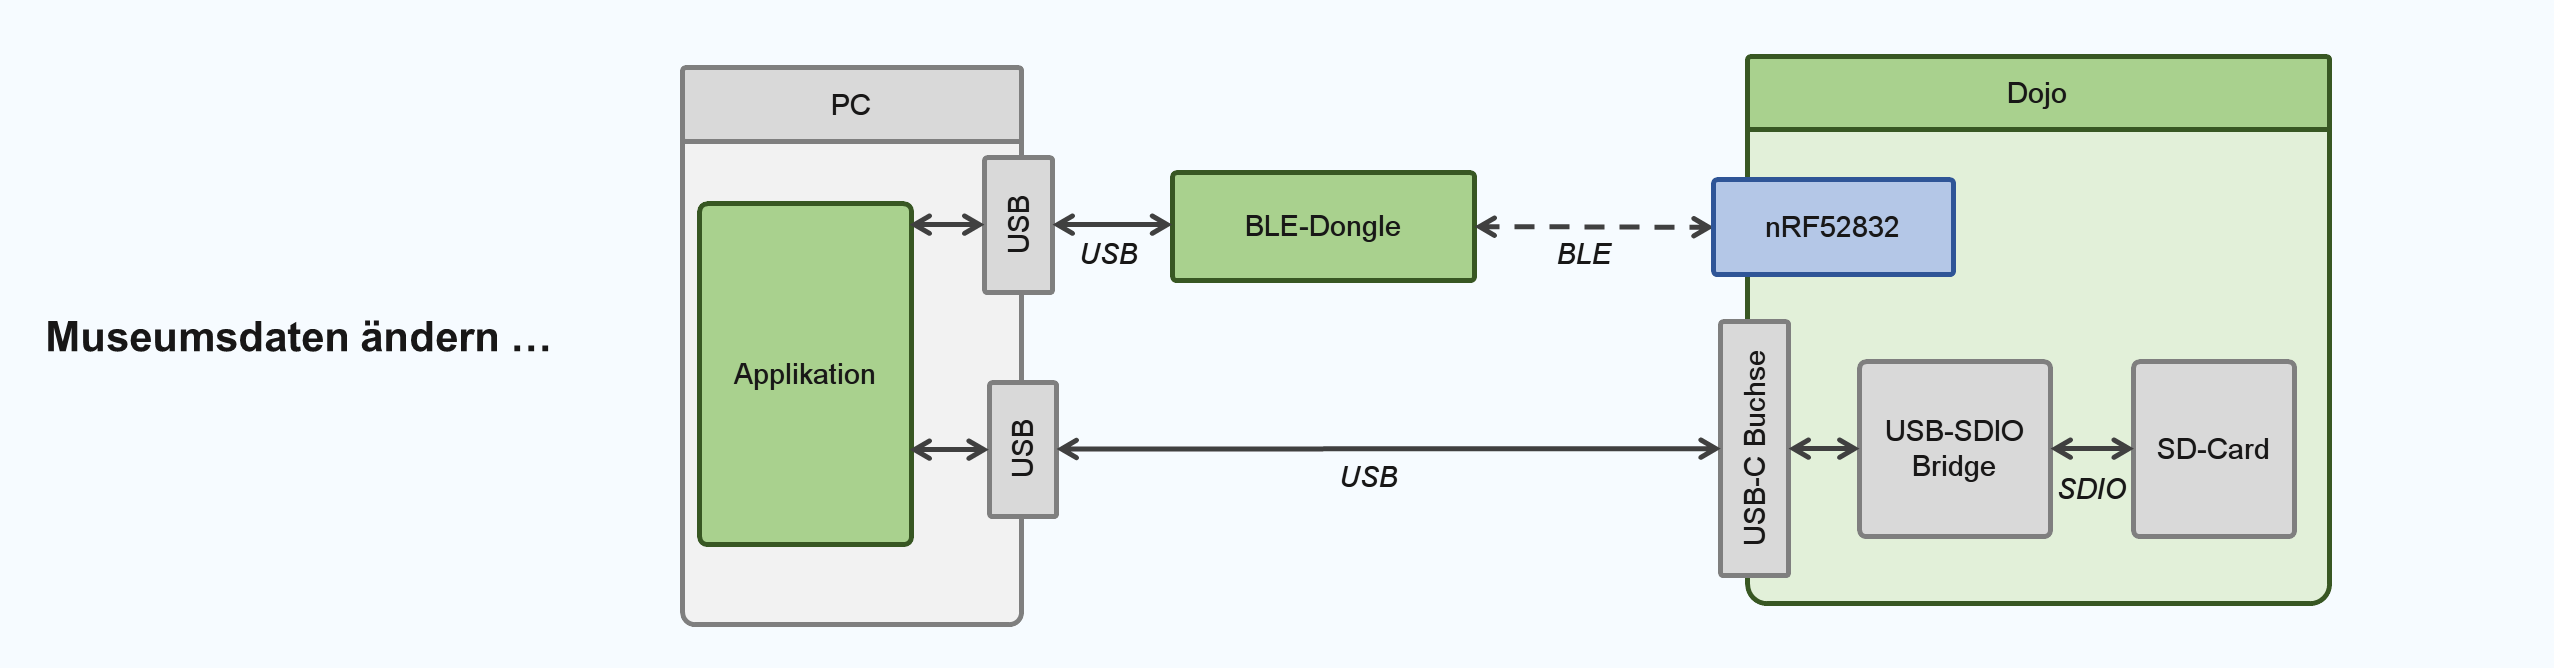
\includegraphics[width=\textwidth]{Zustand_Programmieren.png}
\caption{Zustand beim Programmieren} % picture caption
\label{fig:image3}
\end{figure}

Der zweite Kommunikationskanal wird via BLE realisiert und dient zur Konfiguration des Dojos. Er wird benötigt, um dem Gerät mitzuteilen, welche Audiodateien zu welchem Beacon gehören.\\
\\
In der Abbildung \ref{fig:image2} wird der Zustand Laden dargestellt. Dabei wird das Dojo über die USB-C Buchse mit einem Netzteil verbunden.

\begin{figure}[htb]
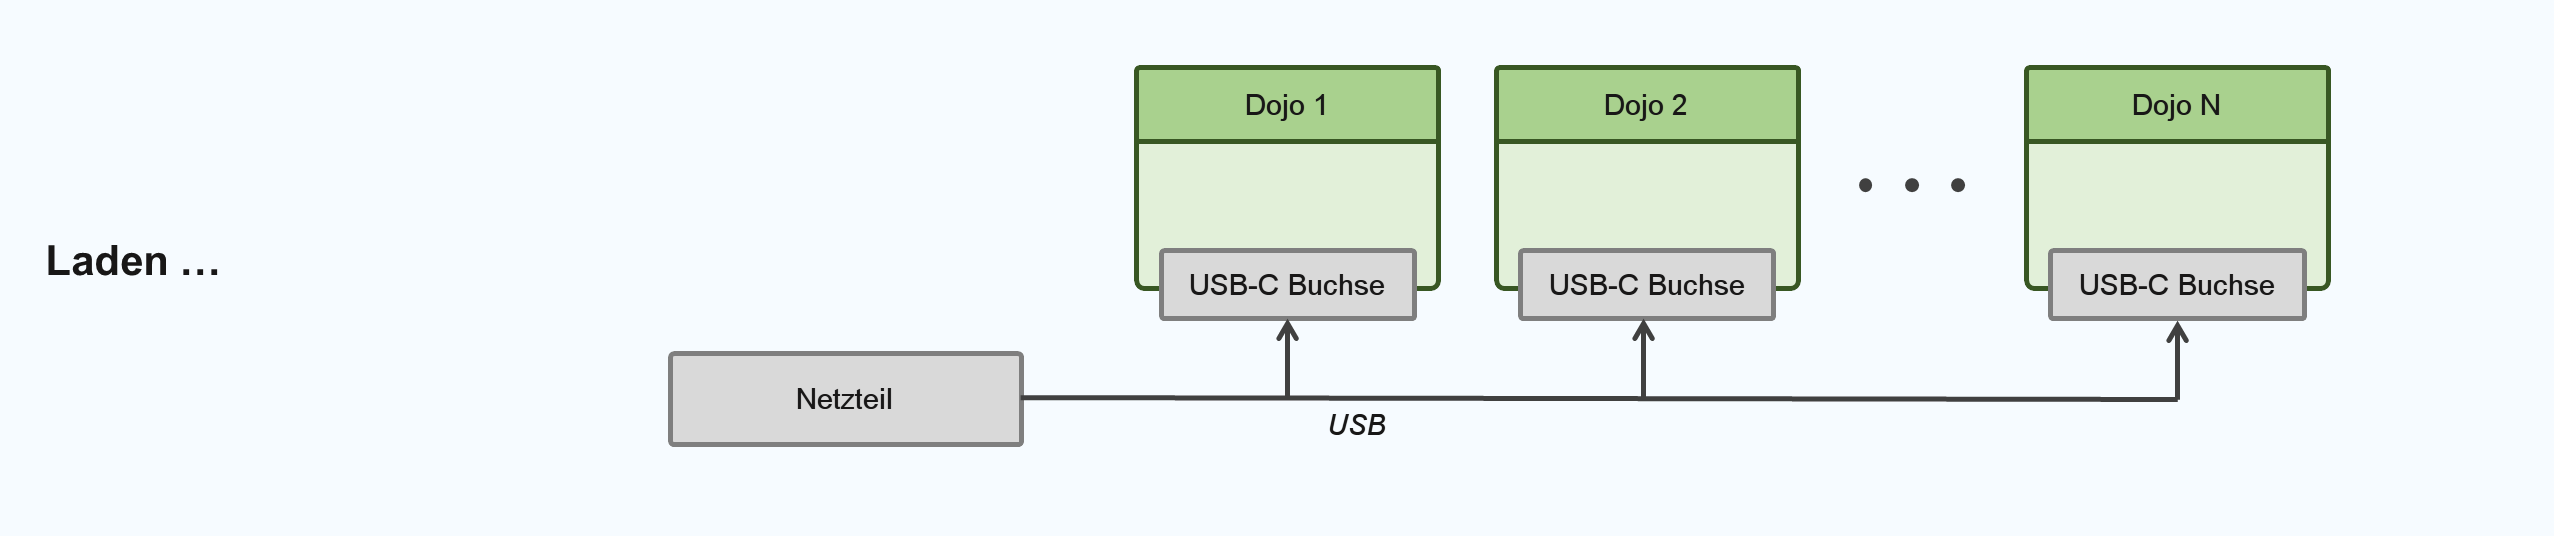
\includegraphics[width=\textwidth]{Zustand_Laden.png}
\caption{Zustand beim Laden} % picture caption
\label{fig:image2}
\end{figure}

Der dritte Zustand (Abb. \ref{fig:image1}) beschreibt wie beim Ein- und Auschecken eines Museumsbesuchers Daten zwischen dem PC des Museums und des Dojos ausgetauscht werden. Dabei handelt es sich um Sprach- und Zutrittseinstellungen. Wie auf der Abbildung \ref{fig:image1} ersichtlich wird ein USB-Donlge benötigt, welcher am PC einzustecken ist. Anhand dieses Dongles weiss das Dojo, dass nun Daten mit einem PC ausgetauscht werden und kann so entsprechende Programmfunktionen aufrufen.
\newpage

\begin{figure}[htb]
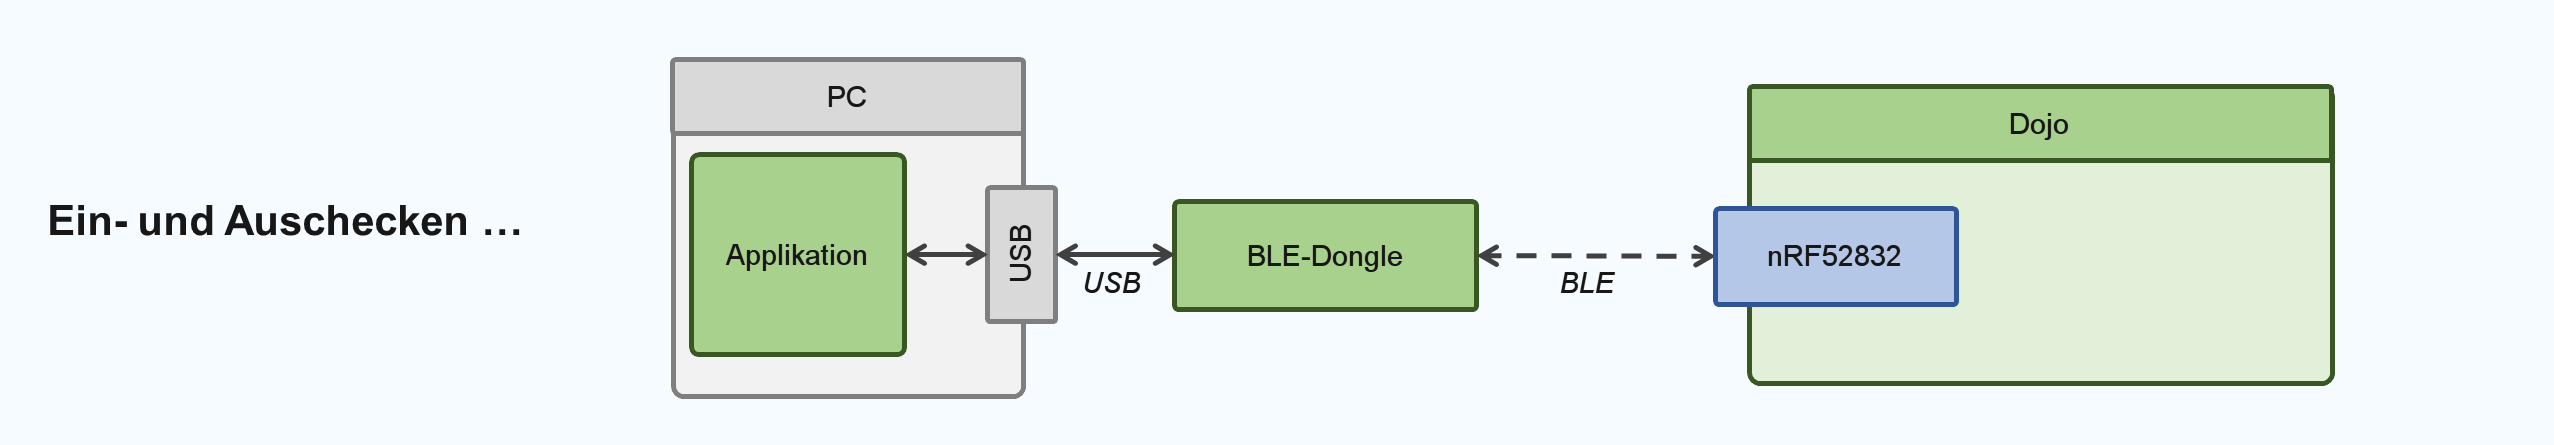
\includegraphics[width=\textwidth]{Zustand_Ein_Aus_Checken.png}
\caption{Zustand beim Ein- und Auschecken} % picture caption
\label{fig:image1}
\end{figure}

Die Abbildung \ref{fig:image4} zeigt den Zugstand beim Rundgang. Die Kommunikation zwischen den Beacons und dem Dojo erfolgt via BLE. Sobald sich der Benutzer einem Kunstwerk nähert, vibriert das Dojo zur Bestätigung. Nun lässt sich das zum Kunstwerk gehörende Audiofile abspielen und es ist dem Besucher möglich dieses zu Liken. Das Kunstwerk bestätigt dies und gibt ein kurzes Feedback. \\
Möchte der Besucher den Museumsbereich wechseln, so muss er eine Schranke passieren. Durch Berühren des Zutrittssystems mit dem Dojo wird diese Schranke geöffnet oder bleibt geschlossen.

\begin{figure}[htb]
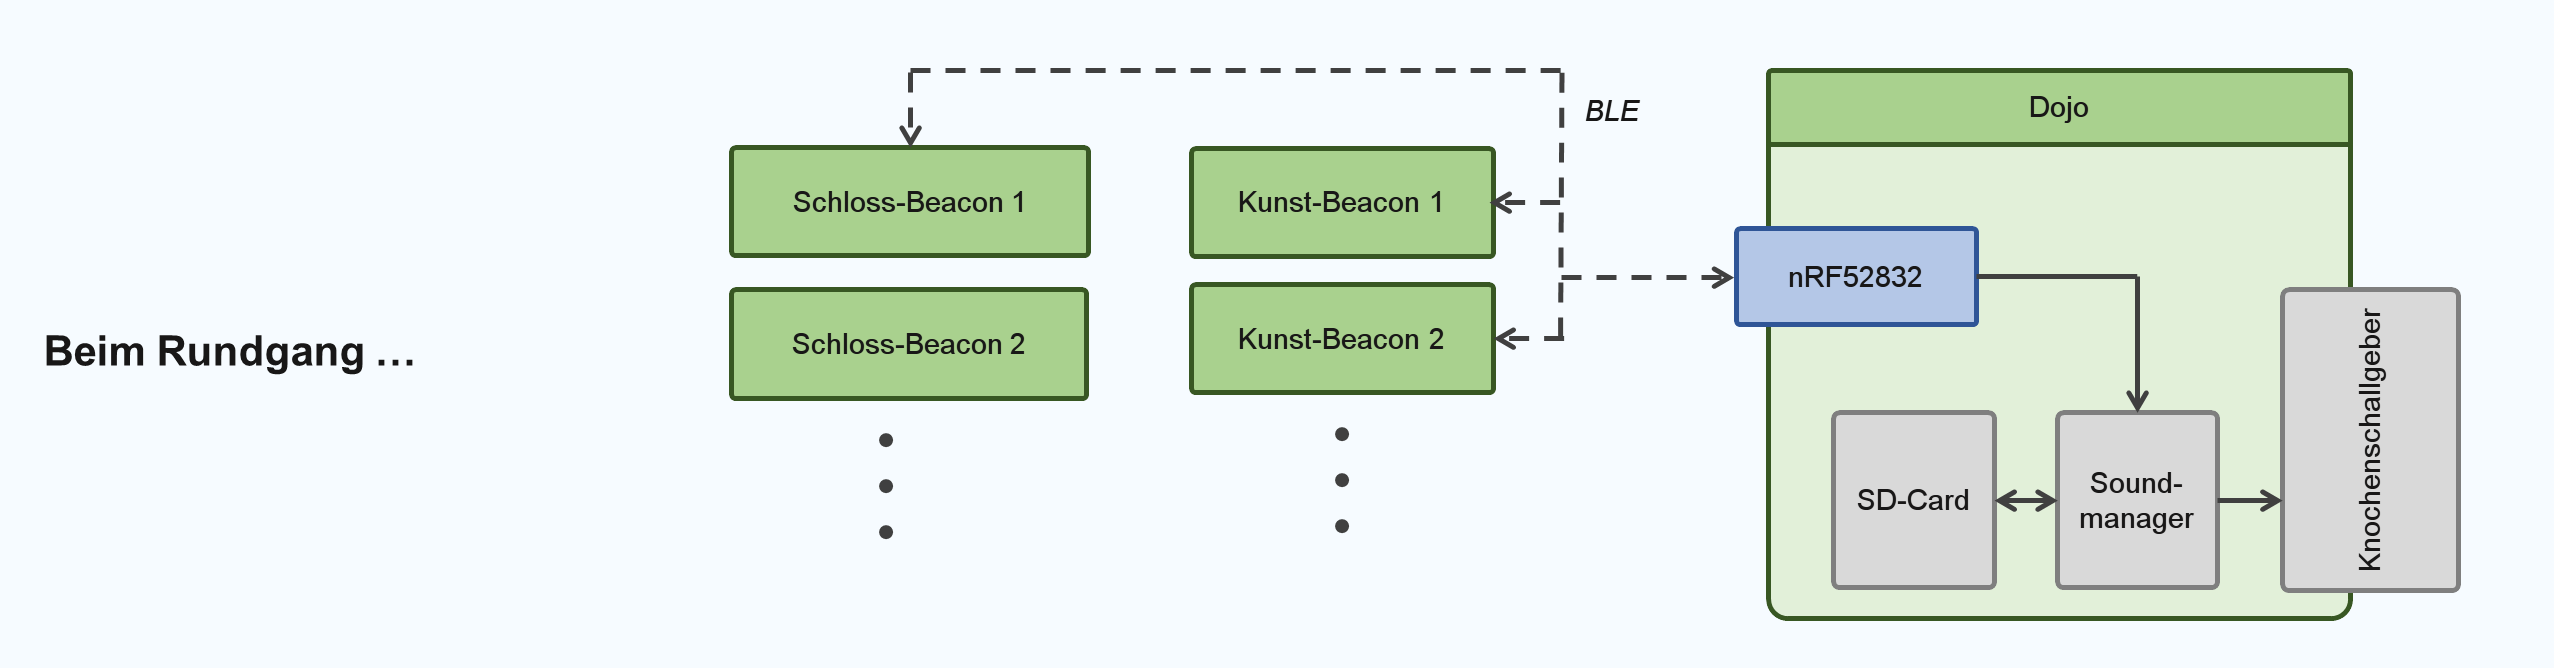
\includegraphics[width=\textwidth]{Zustand_Rundgang.png}
\caption{Zustand beim Rundgang} % picture caption
\label{fig:image4}
\end{figure}

\newpage

%%%%%%%%%%%%%%%%%%%%%%%%%%%%%%%%%%%%%%%%%%%%%%%%%%%%%%%%%%%%%%%%%%%%%%%%%%%%%%%%
\subsection{Hardware} \label{sec:hardware}

Dieser Abschnitt geht auf die in diesem Projekt verbaute Hardware ein. In der Abbildung \ref{fig:dojo} sind die wichtigsten Verbindungen zwischen den Komponenten und deren Abhängigkeit aufgezeigt.

\begin{figure}[htb]
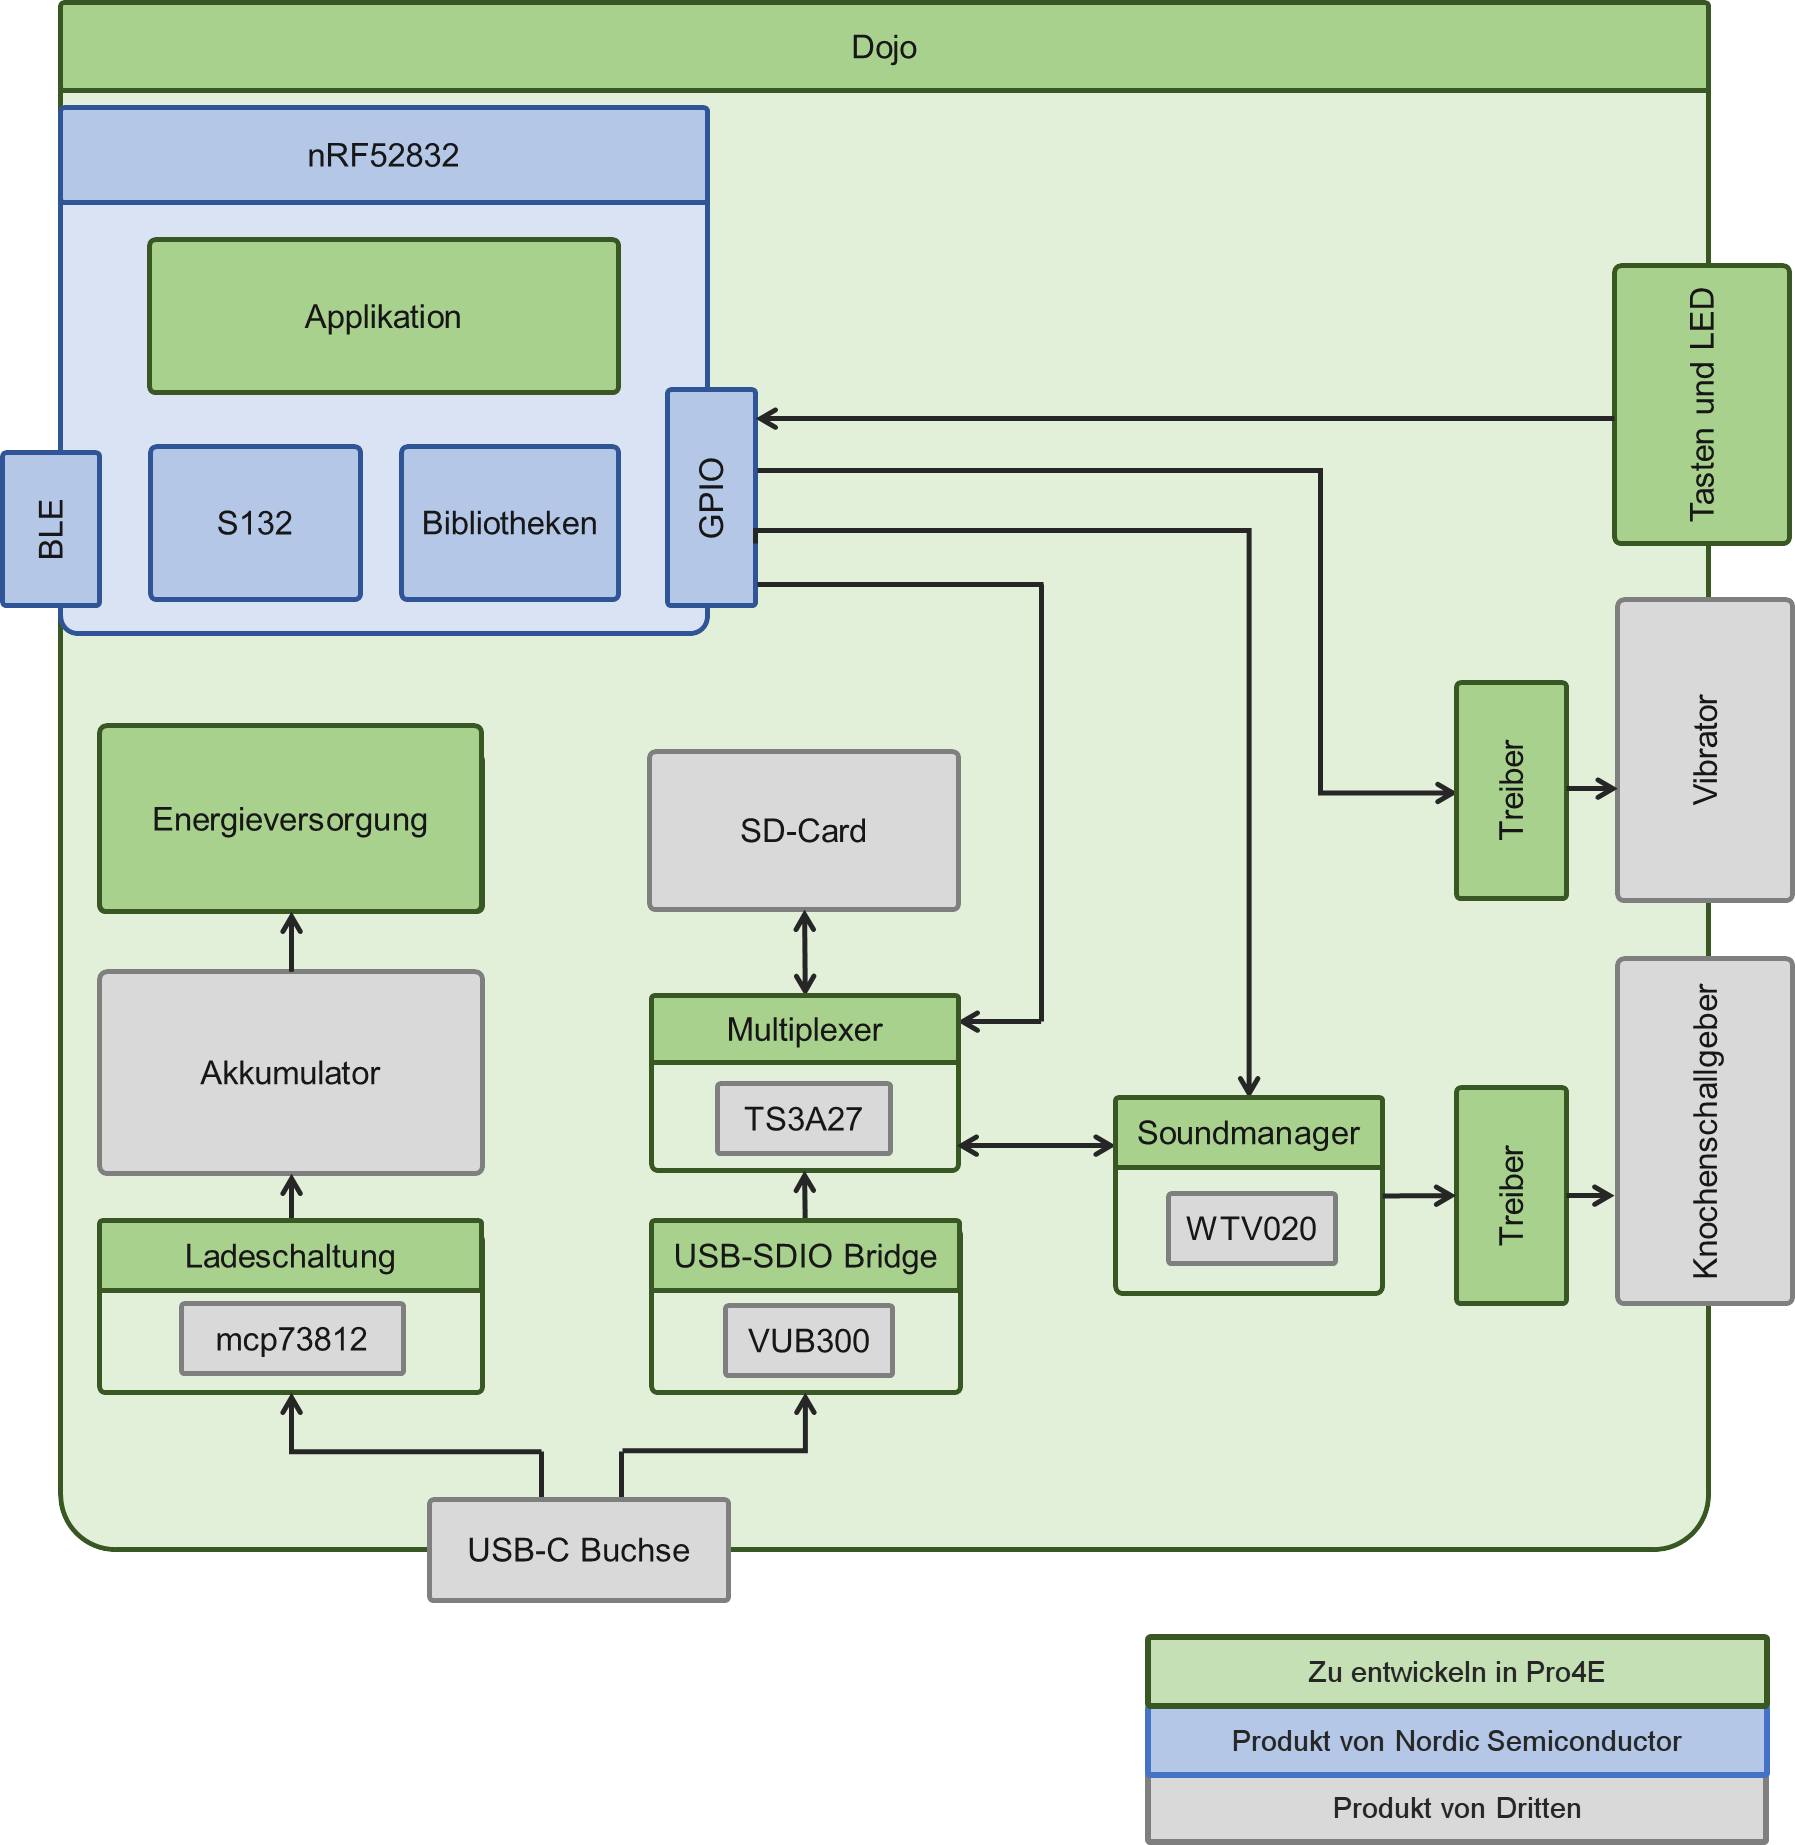
\includegraphics[width=\textwidth]{Dojo.png}
\caption{Übersicht der Hardwarekomponennten des Dojo} % picture caption
\label{fig:dojo}
\end{figure}

\subsubsection{Energieversorgung}
Wie in der Abbildung \ref{fig:image2} ersichtlich bezieht die Elektronik des Dojos ihre Energie aus einem Akkumulator. Verwendet wird ein Lithiumakkumulator mit einer Nennspannung von 3.7V. Dieser soll mindestens eine Kapazität von 0.55Ah haben (siehe Berechnung \ref{eq:equation1}). Mittels eines Spannungsreglers wird aus der Akkumulatorspannung eine stabile Arbeitsspannung erzeugt. Geladen wird das Dojo über die USB-C Buchse. Der Ladestrom wird mithilfe des Ladechips mcp73812 (gem. Datenblatt \cite{MCP73811}) auf 0.5A begrenzt. Die Ladezeit liegt somit unter 6h.\\
\\
\textbf{Berechnung Akkumulatorkapazität:}\\
Das Dojo soll mit einer Akkuladung 8h im Einsatz sein. Als grösster Energieverbraucher wird der Knochenschallgeber eingeschätzt. Während dem Gebrauch in der Ausstellung wird für diesen eine mittlere Leistung von 0.2W angenommen. Wird der Knochenschallgeber mit 3V angesteuert (tiefste in Frage kommende Arbeitsspannung), muss der Akkumulator eine Kapazität von mindestens 0.55Ah haben, ersichtlich in der Berechnung \ref{eq:equation1}.

% equation
\begin{equation}
Q_{min} = \frac{P \cdot t_{Einsatz}}{U} = 0.533Ah \approx 0.55Ah
\label{eq:equation1}
\end{equation}
\begin{tabbing}
\hspace{20mm}	\=  \hspace{60mm} \= \hspace{30mm}	\= 	\\
mit	\\
$Q_{min}$	\> Minimale Akku Kappazität	\> 0.55 Ah	\>	\\
$P$		\> Mittlere Leistung		\> 0.2 W \>	\\
$t_{Einsatz}$	\> Einsatzzeit			\> 8 h	\\
$U$		\> Spannung			\> 3 V	\\
\end{tabbing}

\subsubsection{BLE-Schnittstelle und Mikrokontroller}
Die BLE-Schnittstelle wird mit dem Mikrokontroller nRF52832 (siehe Datenblatt \cite{NRF52832}) realisiert. Der nRF52832 liefert die gesamte BLE hardware ''oneboard'', somit werden keine zusätzlichen Komponenten diesbezüglich benötigt. Dieser Mikrokontroller dient zudem als Steuereinheit für das Dojo. Auf die dabei verwendete Software wird im Abschnitt \ref{sec:software} weiter eingegangen.

\subsubsection{Soundwiedergabe} \label{sec:sound}
Wie auf der Abbildung \ref{fig:image4} ersichtlich dient der Chip WTV020 (siehe Datenblatt \cite{WTV020}) als Soundmanager. Er liest die auf der SD-Karte abgespeicherten Audio-Dateien selbstständig ein und gibt ein entsprechendes PWM-Signal aus. Dieses kann dann mit einer Treiberschaltung verstärkt und an den Knochenschallgeber ausgegeben werden. Gesteuert wird der Soundmanager vom  Mikrokontroller.

\subsubsection{USB-Schnittstelle}
Um Audiodateien auf das Dojo zu laden, wird es über USB 2.0 mit einem Computer verbunden. Dank der USB-SDIO Bridge, welche mit dem Chip VUB300 (siehe Datenblatt \cite{VUB300}) realisiert wird, kann eine PC-Applikation auf die SD-Karte, wie auf ein Laufwerk, zugreifen.

\subsubsection{Speicher}\label{sec:speicher}
Auf dem Dojo befinden sich zwei nichtflüchtige Speichersysteme.  Zum einen wird auf einer SD-Karte die zu den Kunstwerken gehörenden Audiofiles abgespeichert. Aufgrund des Verwendeten Audiochips \ref{sec:sound} kann maximal eine SD-Karte der Grösse 2GB verwendet werden und es können maximal 512 verschiedene Audiofiles darauf abgespeichert werden.\\
Die Informationen, welche Datei zu welchem Kunstwerk gehört, welche Sprache gerade aktiv ist, welche Kunstwerke geliket wurden sowie zu welchen Zonen der Besucher zutritt hat, werden im internen nichtflüchtigen Speicher vom Mikrokontroller abgespeichert. Auf die SD-Karte können sowohl der Soundmanager und die USB-SDIO Bridge zugreifen. Um den Zugriff zu regeln wird ein Multiplexer benötigt. Dafür wird der TS3A27 (siehe Datenblatt \cite{TS3A27518E}) verwendet. Umgeschaltet wird dieser vom Mikrokontroller, sobald eine USB-Verbindung detektiert wird.

\subsubsection{Übrige Peripherie}
Dieses besteht aus Tasten und LEDs nach den Vorgaben aus dem Dojo-Design und einem kleinen Vibrator, welcher den Besucher darüber informiert, dass er sich einem neuen Kunstwerk genähert hat. Angesteuert und verarbeitet werden diese Komponenten durch den Mikrokontroller.

%%%%%%%%%%%%%%%%%%%%%%%%%%%%%%%%%%%%%%%%%%%%%%%%%%%%%%%%%%%%%%%%%%%%%%%%%%%%%%%%
\subsection{Software} \label{sec:software}

Die Software des Dojos wird grob aus drei unabhängigen Modulen bestehen (Abb. \ref{fig:grobkonzept}): einem Hauptprogramm, einem Modul für das Management der Bluetooth-Beacons und einem Modul zur Audioverarbeitung. Das Bluetooth-Modul wird auf dem gleichen Chip wie das Hauptprogramm realisiert und ist nur softwaremässig als getrennt zu betrachten, hingegen wird die Audioverarbeitung separat ausgeführt und ist somit auch physikalisch ausgelagert.

\begin{figure}[htb]
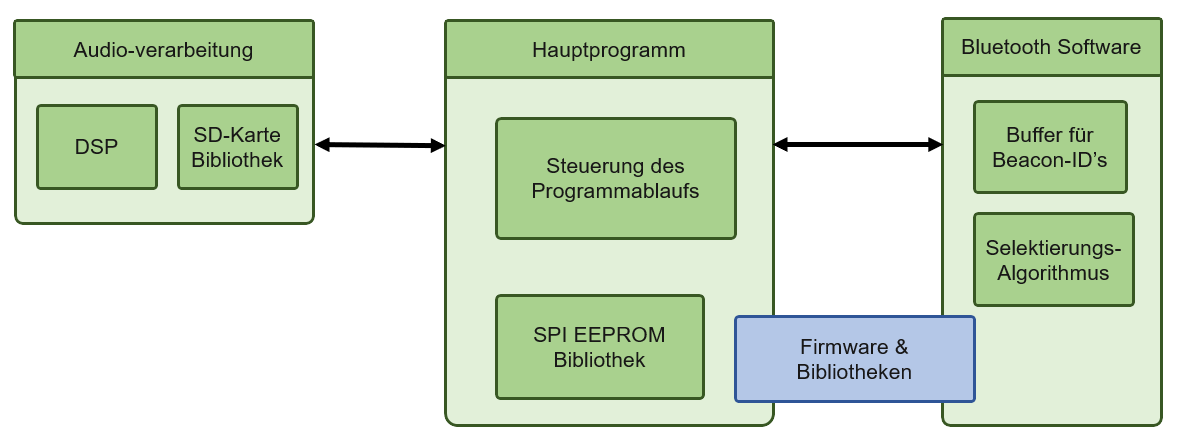
\includegraphics[width=\textwidth]{grobkonzept_software.png}
\caption{Grobkonzept der Firmware des Dojo's} % picture caption
\label{fig:grobkonzept}
\end{figure}

Das Bluetooth-Modul hat die Aufgabe, die IDs aller empfangenen Beacons über eine bestimmte Dauer zu speichern und anhand der Signalstärke den Beacon auszuwählen, welcher sich am nächsten zum Dojo befindet.Dem Hauptprogramm wird signalisiert, wenn sich eine neue ID als stärkste Sendequelle erweist.\\
\\
Das Hauptprogramm steuert den gesamten Softwareablauf, damit sich das Dojo in allen Situationen so verhält, wie es gemäss der Aufgabenstellung soll. werden wie in Abschnit \ref{sec:speicher} erwähnt auf dem internen nichtflüchtigen Speicher abgelegt.\\
\\
Das Audio-Modul erhält vom Hauptprogramm befehle, um Audiodateien abzuspielen oder zu pausieren. Diese wiederum werden von der SD-Karte gelesen. Rückwirkend auf das Hauptprogramm wird es seinen eigenen Status mitteilen und so den Programmablauf beeinflussen.

\subsubsection{Mikrokontroller}
Für dieses Projekt kommt der nRF52832 zum Einsatz. Alle Programme und Treiber für diesen Mikrokontroller, im Zusammenhang mit diesem Projekt, sind in C geschrieben.\\
\\
\textbf{Softdevice}\\
Die Firma Nordic bietet, zur vereinfachten Programmierung ihrer Mikrokontroller, ein umfassendes Software Development Kit (SDK) an. Dieses umfasst diverse Softdevices, Treiber und Softdevices. Für dieses Prjekt wird das Softdevice S132 verwendet.\\
\\
\textbf{Treiber}\\
\\
Es werden für die folgenden Hardwarekomponenten Treiber geschrieben, damit diese mit dem Mikrokontroller angesteuert werden können (Infos zur Hardware in Kapitel \ref{sec:hardware}):
\begin{itemize}
	\item{Multiplexer}
	\begin{itemize}
		\item{Multiplexer Ein/- und Ausschalten}
	\end{itemize}
\end{itemize}

\begin{itemize}
	\item{Audiointerface}
	\begin{itemize}
		\item{Play,Pause,Stop,Songauswahl und Lautstärke regeln}
	\end{itemize}
\end{itemize}

\begin{itemize}
	\item{BLE}
	\begin{itemize}
		\item{Detektion von BLE-Beacons und Informationsaustausch mit diesen}
	\end{itemize}
\end{itemize}

\begin{itemize}
	\item{Flash EEPROM}
	\begin{itemize}
		\item{Lesen und Schreiben}
	\end{itemize}
\end{itemize}

\begin{itemize}
	\item{Datenprüfung}
	\begin{itemize}
		\item{Kontrollieren ob Daten korrekt geladen/gelöscht}
	\end{itemize}
\end{itemize}

%%%%%%%%%%%%%%%%%%%%%%%%%%%%%%%%%%%%%%%%%%%%%%%%%%%%%%%%%%%%%%%%%%%%%%%%%%%%%%%%
% Bedienung
%%%%%%%%%%%%%%%%%%%%%%%%%%%%%%%%%%%%%%%%%%%%%%%%%%%%%%%%%%%%%%%%%%%%%%%%%%%%%%%%
\section{Bedienung}\label{sec:bedienung}
%%%%%%%%%%%%%%%%%%%%%%%%%%%%%%%%%%%%%%%%%%%%%%%%%%%%%%%%%%%%%%%%%%%%%%%%%%%%%%%%
\subsection{Bedienung des Dojos}
Die Bedienung des Dojos erfolgt über die Tasten auf der Oberseite des Dojos (gem. Abbildung \ref{fig:dojointerface}). Diese ermöglicht es dem Museumsbesucher über die Play/Pause-Taste, das zum gerade betrachteten Kunstwerk passende Audiofile abzuspielen. Über die Plus/Minus-Taste kann die Lautstärke der Audiowiedergabe verstellt werden. Die Möglichkeit, mittels Tasten Power Ein/Aus und Vibro Ein/Aus entsprechen ihrer Funktion. Abschliessend besteht die Möglichkeit mittels des Like-Buttons auf der Unterseite des Dojos das bevorzugte Kunstgegenstände zu Liken. Dies ermöglicht es dem Kunden an der Kasse ergänzende Literatur über die von ihm gelikten Kunstgegenstände zu erhalten.

\begin{figure}[htb]
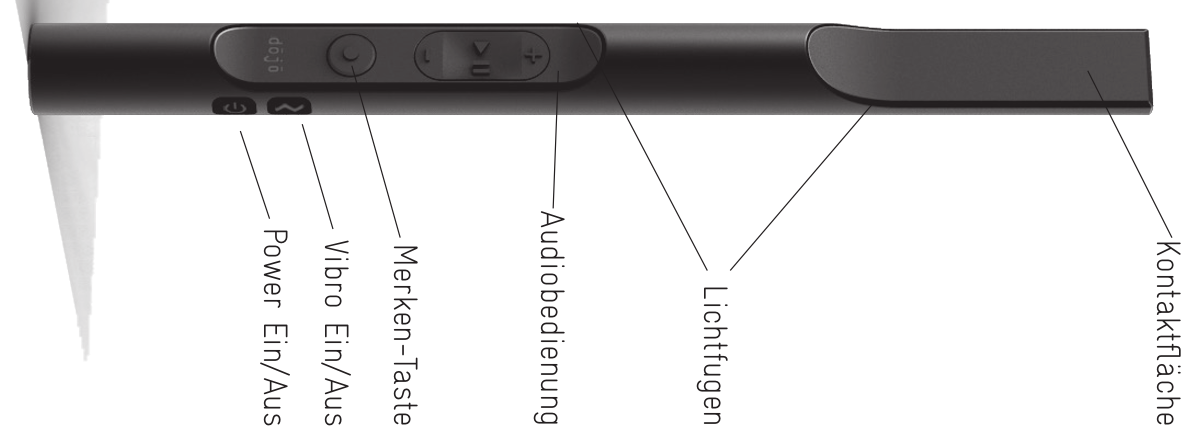
\includegraphics[width=\textwidth]{dojointerface.png}
\caption{Userinterface des Dojo \cite{DOJO}} % picture caption
\label{fig:dojointerface}
\end{figure}

\newpage

\subsection{Bedienung der Testapplikation}
Damit bereits in einer ersten Phase Daten und Audiofiles auf das Dojo geladen werden können, steht eine Java-Applikation zur Verfügung (siehe Abb. \ref{fig:testaplikation}). Diese ermöglicht es dem Museumspersonal, aus einer Bibliothek von Audio-Files, zusätzliche Daten auf das Dojo zu laden oder bestehende zu löschen. Weiter kann, wie auf der linken Seite ersichtlich, die Sprache der Ausgabe eingestellt werden und eventuelle Zutrittseinschrenkungen festgelegt werden. Links unten steht weiter noch ein Feld zur Verfügung, über welches die Audiofiles am PC abgespielt werden können.

\begin{figure}[htb]
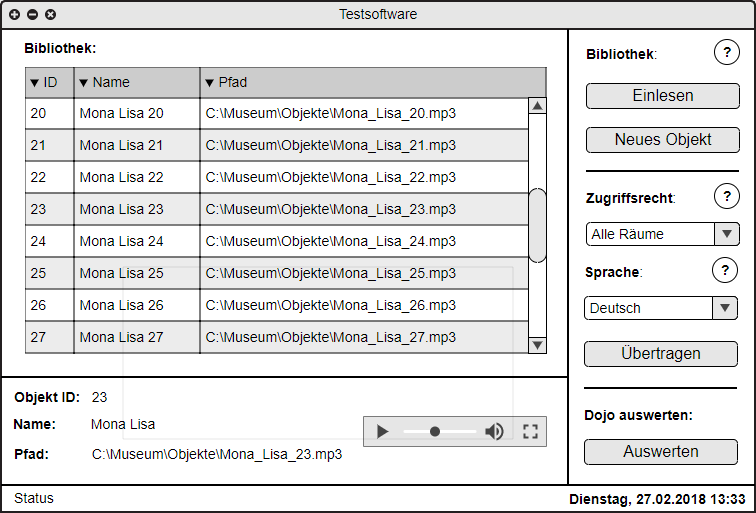
\includegraphics[width=\textwidth]{Testsoftware.png}
\caption{Userinterface der Testaplikation} % picture caption
\label{fig:testaplikation}
\end{figure}


%%%%%%%%%%%%%%%%%%%%%%%%%%%%%%%%%%%%%%%%%%%%%%%%%%%%%%%%%%%%%%%%%%%%%%%%%%%%%%%%
% Testkonzept
%%%%%%%%%%%%%%%%%%%%%%%%%%%%%%%%%%%%%%%%%%%%%%%%%%%%%%%%%%%%%%%%%%%%%%%%%%%%%%%%
\section{Testkonzept}\label{sec:testkonzept}
%%%%%%%%%%%%%%%%%%%%%%%%%%%%%%%%%%%%%%%%%%%%%%%%%%%%%%%%%%%%%%%%%%%%%%%%%%%%%%%%
Zur Validierung des Produkts wird die Firmware auf einem nRF52832 Development Kit entwickelt und getestet. Dieses Board verfügt neben diversen Peripheriegeräten auch einen SEGGER J-Link Debugger. Dieser erlaubt es, die Software direkt auf der Hardware zu debuggen (anstatt nur in einer Simulation der Entwicklungsumgebung).\\
\\
Bluetooth-Beacons können mit geringem Aufwand von bluetoothfähigen Geräten wie Notebooks oder Handys simuliert werden. Somit kann einfach eine Simulationsumgebung erschaffen werden, welche die Situation im Museum nachahmt. Nordic Semiconductors, der Hersteller des verwendeten Mikrocontrollers, stellt ausserdem eine vielzahl von Apps für die Verwendung, Simulation und Analyse von Bluetoothverbindungen und Dienste zur Verfügung. Damit lässt sich auch das Verhalten der Gegenseite (Feedback der Beacons und die Zutrittskontrolle) zum Dojo testen. Die Testsoftware, in diesem Falle eine Java-Applikation, kann direkt in diese Simulationsumgebung einbezogen werden.\\
\\
Mit dieser Testsoftware kann die auf dem Dojo befindliche Bibliothek mit Museumsobjekten aktualisiert werden, sowie Museumsbesucher-Einstellungen wie beispielsweise die gewünschte Sprache übertragen werden kann. Die Daten der Museumsobjekte selbst befinden sich ausgelagert in einer .xml Datei auf dem Computer, welche von der Java-Applikation leicht eingelesen werden kann. Durch diese Auslagerung der Daten kann der Museumsbetreiber ohne eine Anpassung der Software neue Museumsobjekte erstellen und Besuchereinstellungen erweitern.

%%%%%%%%%%%%%%%%%%%%%%%%%%%%%%%%%%%%%%%%%%%%%%%%%%%%%%%%%%%%%%%%%%%%%%%%%%%%%%%%
% bibliography
%%%%%%%%%%%%%%%%%%%%%%%%%%%%%%%%%%%%%%%%%%%%%%%%%%%%%%%%%%%%%%%%%%%%%%%%%%%%%%%%
\section{Bibliographie}\label{sec:bibliographie}
\bibliography{01_bibliography}
\clearpage

\end{document}
